\section{Methods}
\label{sec:methods}

\subsection{Threat model}
We consider the following adversaries.
\begin{description}
	\item[Network-level adversary] An adversary that monitors at least
		one autonomous system, e.g., ISP, VPS provider, government.
	\item[Relay-level adversary] An adversary that runs at least one Tor relay.
	\item[DNS provider] An adversary that operates the DNS resolver used
		by exit relays, e.g., Google.
	\item[Active] To which extent to we consider active, content-modifying
		adversaries?  Attackers that see DNS can poison response and redirect
		victim to attacker-controlled domain.  That turns problem into trivial,
		classical end-to-end correlation.  Still, probably reason enough to tell
		exit relays that they should use DNSSEC.  Also, we might spot these
		attacks using exitmap.
\end{description}

We do not consider the case where Tor users misconfigure their client and leak
DNS requests unintentionally.

\subsection{Exposure at the Guard side}
\begin{itemize}
	\item Bad guards
	\item recognise dns requests by traffic analysis on the wire.  probably
		difficult because of optimistic data?  can we do more than just timing?
	\item can flow watermarking help?  see houmansadr's
		work~\cite{Houmansadr2011a}
\end{itemize}

\subsection{Internet map}
\begin{itemize}
	\item Where do we get our AS and IXP graph from?
	\item Johnson et al.~\cite[\S 5.2]{Johnson2013a} used RouteViews and the CAIDA IPv4
		Routed /24 AS Links Dataset, resulting in 44,605 ASs connected by
		305,381 links.
\end{itemize}

\subsection{Traceroute dataset}
\label{sec:traceroute-dataset}
\begin{itemize}
	\item Find machines that are topologically close to DNS resolvers
		used by exit relays.
	\begin{itemize}
		\item RIPE Atlas probes.
		\item Virtual private systems.
		\item PlanetLab nodes.
		\item Ask exit operators to run traceroutes for us.
	\end{itemize}
	\item Run traceroutes to DNS servers to determine path coverage.
	\item Determine ``AS inflation factor.''
\end{itemize}

In this analysis we assume that an AS that can see traffic entering the Tor network and 
DNS traffic at the other end can use this information in order to deanonymize the 
entering traffic. Here we seek to measure the chances an AS will be in the ``correct'' 
position to carry out such an attack.

A Tor exit can carry out DNS name resolution in two different ways: it can either do it
itself by running a name server locally, or it can rely on a 3rd-party name server, 
such as its ISP's name server or a public DNS name server like Google's 8.8.8.8.

Let us examine these two different scenarios: local resolution vs. 3rd-party 
resolution. With local resolution, a good position for an AS is to be on the path between 
a Tor client and a Tor guard and on the path between a Tor exit and any of the name 
servers the exit has to communicate with in order to resolve the name. These name servers 
can include the root name server, the TLD servers, and the other ones**fix this. The ASes 
along the way from the exit relay to the name servers will be able to see the domain 
names that are being queried.

For 3rd party resolution, a good position for an AS is to be on the path between 
a Tor client and a Tor guard and on the path between the exit relay and that 3rd party 
name server. Beyond that, the queries will look like they're coming from the IP address 
of the name server and not the IP address of the exit relay, which is what we're interested 
in.

In order to do our analysis, we need to have some way of figuring out the AS-level paths. 
We considered two options: the use of AS path inference and the use of traceroute data. 
We decided against AS path inference because Juen et al. showed that it can be quite
inaccurate~\cite{Juen2015a}.  Thus, we decided to go with actual traceroute data. Here,
again, we had to consider our options on how to obtain this data. We considered the
PlanetLab and RIPE Atlas measurement platforms and asking Tor relay operators to run
traceroutes for us.  We decided against using Tor relay operators to run traceroutes for
us because of the inconvenience (Murdoch paper did this and Juen paper did this). We
decided against PlanetLab because its nodes tend to be in university networks. Hence, we
decided to use RIPE Atlas~\cite{atlas}. RIPE Atlas has probes in many ASes that have Tor
relays. As shown in Table~\ref{tab:atlas-coverage}, for a day in May 2016, we found that
RIPE Atlas had probes in 52\% of ASes that contain Tor exit relays.  We found that RIPE
Atlas has probes in 51\% of ASes that contain Tor guard relays. More importantly, we found
that Atlas ASes cover 58\% of Tor exit bandwidth and 74\% of Tor guard bandwidth. This is
important because Tor relay usage is not evenly split among all of the relays. This
coverage is significant because as the Murdoch paper states, ``As Tor does not currently
implement a a mechanism for performing traceroutes, the operator of the node must do so
manually. Furthermore, the Juen paper was only able to cover around 28\% of exit bandwidth
by asking operators to run traceroutes for them.  Thus, we find that RIPE Atlas gives us a
great way to study the paths that Tor circuits might traverse. (I'm wondering if a table
might be better for those percentages .  . .) In order to get our traceroutes, we ran
traceroutes from probes that that were in the same ASes as Tor guards and exits. TODO:
Mention why we picked AS 6128 as our client AS.

% - 197 out of all 377 (52%) Tor exit ASs have Atlas probes.
% - 220 out of all 434 (51%) Tor guard ASs have Atlas probes.

% - Atlas ASs cover 57.53% of Tor exit bandwidth.
% - Atlas ASs cover 73.59% of Tor guard bandwidth.

\begin{table}[t]
	\caption{The coverage of RIPE Atlas nodes that are colocated with Tor guard and exit
	relays.}
	\label{tab:atlas-coverage}
	\centering
	\begin{tabular}{l|r r}
	\toprule
	\textbf{Atlas probe coverage} & \textbf{Tor guard ASs} & \textbf{Tor exit ASs} \\
	\midrule
	By bandwidth & 73.59\% & 57.53\% \\
	By number & 50.69\% & 52.25\% \\
	\bottomrule
	\end{tabular}
\end{table}

We also had to consider what method we'd use to translate the IP addresses in our 
traceroutes to ASes. The options we considered were Team Cymru and pyasn. We decided to 
go with pyasn because it uses actual control plane data in order to perform the 
translations vs. using whois, which is what Team Cymru uses (find source for this). 
(A word of caution: if there is an AS that is annoucing bogons on a particular day, and 
you unluckily happen to pick that day, you might get bogus translations. For example, an 
IP address like 10.10.10.1 might result in an AS number instead of 'None'.)

In order to measure the chances an AS will be in the ``correct'' position to carry out a
deanonymization attack, we make use of TorPS, the Tor Path Simulator. This tool 
``faithfully mimics the behavior of Tor client software for creating exit circuits.''
That is, it gives us realistic combinations of guards and exits based on the state of the 
Tor network for a given time. TorPS is based on Tor version X. For each sample, it uses 
one guard which will expire after 270 days. We have TorPS simulate the behavior of a Tor 
client for the month of March 2016. We use 50,000 samples for the same reasons given in
``Users Get Routed.'' (Should we mention the fixes we made to TorPS? Should we mention 
the problem we found with their user models?) For our simulation, we had each sample 
visit nymity.ch once per hour for the entire month of March 2016. Thus, each sample had 
a total of 744 opportunites to be compromised (this assumes that the circuit changes 
every time the sample/user visits nymity.ch). It is much better to use a tool like TorPS 
in order to measure these chances instead of just using all permutations of guard and 
exits.

In this analysis, we completely ignore caching of any type, so our results are overly 
pessimistic. TODO: Mention that these results apply only to what we had data for: about 
half.

Describe the four scenarios in the graph here: 1) Traditional, 2) Google, 3) Local, and 
4) Status Quo.

Traditional: ``Traditional'' represents the paths between all exit ASes that RIPE Atlas 
has coverage for and nymity.ch. That is, this measurement doesn't take DNS into account 
at all, as has been traditionally done.

Google (8.8.8.8): ``Google'' represents what would happen if all exit relays used 
Google's public DNS server for resolution. We ran traceroutes from probes in all the exit 
ASes that RIPE Atlas had coverage for to 8.8.8.8.

Local: ``Local'' represents what would happen if all exit relays ran their own name 
servers locally (e.g., the use of unbound) on their own machines. In order to figure out 
what ASes would be traversed on the way to resolve nymity.ch. In order to figure out the 
DNS delegation path, we use part of the ddptr tool. Assuming no caching and assuming 
iterative resolution, for nymity.ch the name server will have to visit three name servers:
a root name server, a top level domain name server, and a second level domain name server. 

Status Quo: ``Status Quo'' represents to the best of our ability the type of name resolution 
that exit relays perform, whether that be their own or the use of 3rd-party name servers, 
which again includes public DNS name servers and their ISPs' name servers. To figure this 
out, we used the exitmap tool, our own website, and our own authoritative name server 
in order to figure out the IP addresses of the name servers that the exit relays were 
using. We then performed traceroutes from the exit ASes to the appropriate IP addresses 
in order to get the AS-level paths.

TODO: Get the numbers from my data for the fan-out.

As you can see in Figure~\subref{fig:compromised-streams} and
Figure~\subref{fig:time-until-compromise}, 
Google fared much better than the other situations. This might lead you to believe that 
Tor exit relays should use 8.8.8.8 for all of their name resolution needs, but then you've 
given Google A LOT of power. It might actually be better to tell Tor exit relay operators 
to use their ISPs' default name servers because the ISPs get to see the Tor destinations 
anyway!

The Status Quo results are significantly better than the Local results because only X\% 
of Tor exit relays actually do their own resolution.

\begin{figure}[t]
\centering
\subfigure[The number of compromised streams for March 2016.]{
	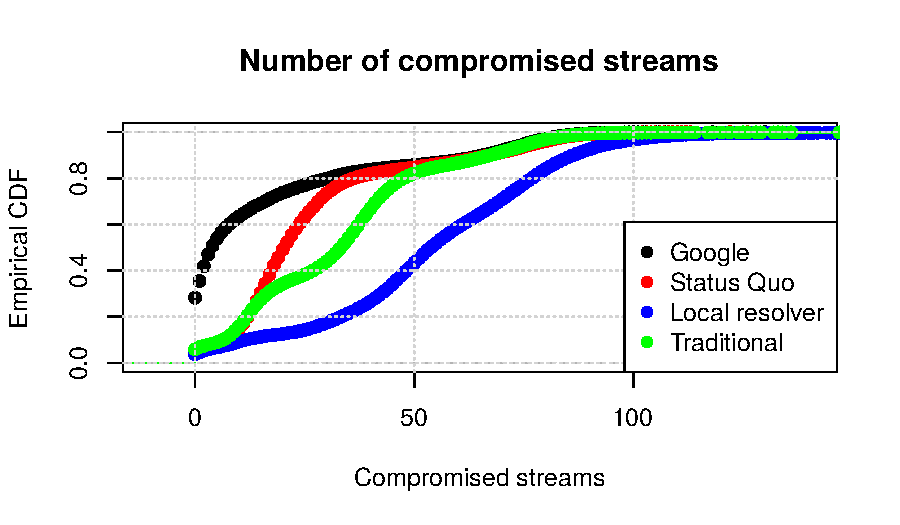
\includegraphics[width=0.466\linewidth]{figures/num-compromised-streams.pdf}
    \label{fig:compromised-streams}
}
\subfigure[The time to first compromise for March 2016.]{
	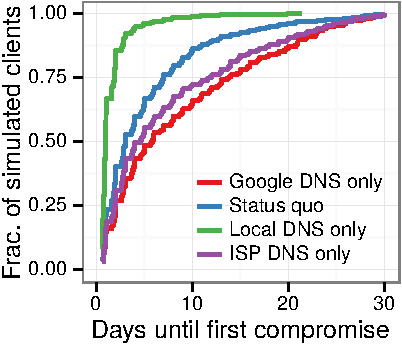
\includegraphics[width=0.466\linewidth]{figures/time-until-compromised.pdf}
    \label{fig:time-until-compromise}
}
\caption{Two simulations for March 2016 that show the number of compromised
	streams (Figure~\subref{fig:compromised-streams}) and the time until the
	first compromised stream (Figure~\subref{fig:time-until-compromise}).}
\label{fig:compromise-stream-time}
\end{figure}

\subsection{DNS packet sizes at entry guard}
\begin{itemize}
	\item Send many DNS requests over entry guard.
	\item Capture them on the wire and look at them.
	\item What's the best way to filter out the noise?
\end{itemize}

\subsection{Practical attacks}
We leverage the following building blocks:
\begin{itemize}
	\item Traffic analysis done on an entry guard.  Can DNS requests be isolated
		reliably?
	\item Access to DNS root, .com, and .net.
	\item Ability to use DNS resolver's cache as an oracle.
	\item Ability to enumerate what resolver's an exit relay uses.
	\item Resolvers using EDNS.
	\item Users in country X are likely to resolve domains of country X.
\end{itemize}
